\subsection*{Fonctions harmoniques}
Résolution similaire aux problèmes bornés.\\
\textbf{Exemple:}\\
On veut résoudre:
\begin{equation*}
    \left\{
    \begin{aligned}
         & u(x,y)=\Delta u=u_{xx}+u_{yy} \\
         & D=\{0<x<a,0<y<b\}             \\
    \end{aligned}
    \right.
\end{equation*}
avec les conditions aux bords:
\begin{figure}[H]
    \centering
    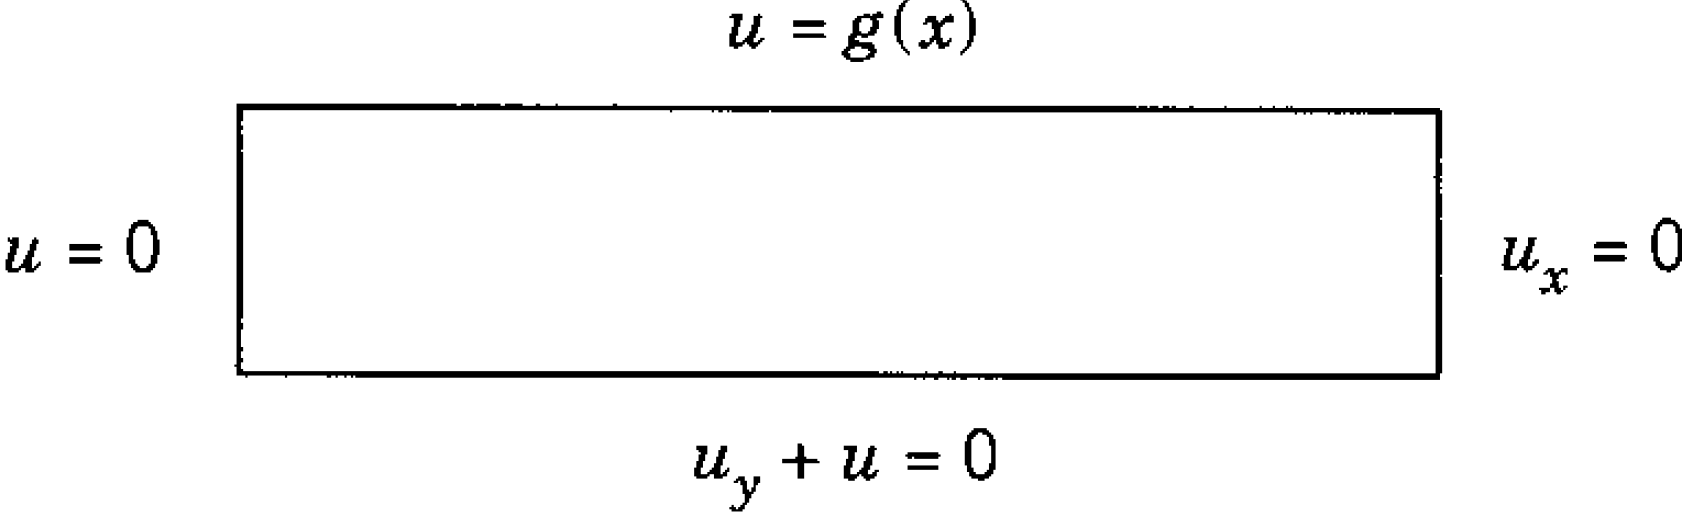
\includegraphics[width=0.75\linewidth]{images/semaine5_condi_bord.png}
\end{figure}
trouver les valeurs propres et les fonctions propres :
\begin{subequations}
    \begin{equation*}
        u(x,y)=X(x)Y(y)\Longrightarrow \frac{X''}{X}+\frac{Y''}{Y}=0
    \end{equation*}
    \begin{equation*}
        \left\{
        \begin{aligned}
             & X''+\lambda X=0 \quad \text{pour} \quad 0\leq x\leq a \\
             & Y''-\lambda Y=0 \quad \text{pour} \quad 0\leq x\leq b \\
        \end{aligned}
        \right.
    \end{equation*}
    \begin{equation*}
        \left\{
        \begin{aligned}
             & \lambda=\beta^2=(n+\sfrac{1}{2})^2\frac{\pi^2}{a^2}                                       \\
             & \colorbox{green}{$X(x)$}=A\cos(\beta x)+B\sin(\beta x)=\colorbox{green}{$B\sin(\beta x)$} \\
             & \text{car} \quad X(0)=X'(a)=0
        \end{aligned}
        \right.
    \end{equation*}
    \begin{equation*}
        \left\{
        \begin{aligned}
             & \colorbox{yellow}{$Y(y)$}=A\cosh(\beta y)+B\sinh(\beta y)=\colorbox{yellow}{$\beta\cosh(\beta y)-\sinh(\beta y)$} \\
             & \text{car} \quad Y'(0)+Y(0)=C+D\beta=0 \Longrightarrow D=-1 \quad \text{et} \quad C=\beta                         \\
        \end{aligned}
        \right.
    \end{equation*}
\end{subequations}
il reste à sommer la série est trouver $g(x)$
\begin{subequations}
    \begin{equation*}
        u(x,y)=\sum_{n=0}^{\infty}\colorbox{green}{$B_n\sin(\beta_nx)$}\colorbox{yellow}{$(\beta_n\cosh(\beta_ny)-\sinh(\beta_ny))$}
    \end{equation*}
    \begin{equation*}
        u(x,b)=g(x)=\sum_{n=0}^{\infty}\underbrace{B_n(\beta_n\cosh(\beta_nb)-\sinh(\beta_nb))}_{E_n}\sin(\beta_nx)
    \end{equation*}
\end{subequations}
\textbf{Formule de poissons:}\\
On veut séparer les variables en coordonnées polaires $u=R(r)\Theta(\theta)$:
\begin{equation*}
    u_{xx}=+u_{yy}=u_{rr}+\frac{1}{r}u_r+\frac{1}{r^2}u_{\theta\theta}
\end{equation*}
puis on procède comme d'habitude.
